\part*{附録\three}
\addcontentsline{toc}{part}{\texorpdfstring{附録\three}{附録\three}}


\section*{p228:問}
\addcontentsline{toc}{section}{\texorpdfstring{p228:問}{p228:問}}

\subsection*{p228:問-(イ)}
\addcontentsline{toc}{subsection}{\texorpdfstring{p228:問-(イ)}{p228:問-(イ)}}
以下により,求める最大公約数は$x^2+x-1$である.

\begin{figure}[ht]
  \centering
  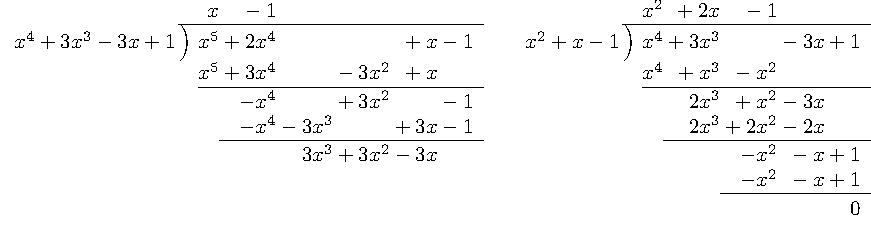
\includegraphics{emath_figures/p228_toi_i.pdf}
\end{figure}


\subsection*{p228:問-(ロ)}
\addcontentsline{toc}{subsection}{\texorpdfstring{p228:問-(ロ)}{p228:問-(ロ)}}

以下により,これらは互いに素である.

\begin{figure}[ht]
  \centering
  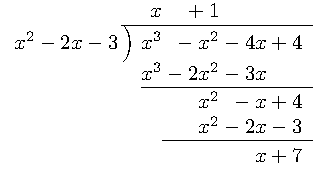
\includegraphics{emath_figures/p228_toi_ro.pdf}
\end{figure}



\section*{p239:問1}
\addcontentsline{toc}{section}{\texorpdfstring{p239:問1}{p239:問1}}

\subsection*{p239:問1-(イ)}
\addcontentsline{toc}{subsection}{\texorpdfstring{p239:問1-(イ)}{p239:問1-(イ)}}


\begin{tanswer}
  計算すると以下のようになる:
  \begin{align*}
    {x_1}^2 + {x_2}^2+\dots+{x_n}^2 & = \left (\sum_{i=1}^{n} x_i \right )^2 - 2\sum_{1\leqq i < j \leqq n} x_j x_k \\
                                    & = (x_1+x_2+\dots+x_n)^2 - 2(x_1 x_2 + x_1 x_3 + \dots + x_{n-1} x_n)
                                    & = s_1^2 - 2s_2.
  \end{align*}
\end{tanswer}


\subsection*{p239:問1-(ロ)}
\addcontentsline{toc}{subsection}{\texorpdfstring{p239:問1-(ロ)}{p239:問1-(ロ)}}
\begin{tanswer}
  計算すると以下のようになる:
  \begin{align*}
    {x_1}^3 + {x_2}^3+\dots+{x_n}^3 & = \left (\sum_{i=1}^{n} x_i \right )^3 - 3\left (\sum_{i=1}^{n} x_i \right ) \left(\sum_{1 \leqq i <j \leqq n} x_i x_j \right) + 3\sum_{1\leqq i < j < k \leqq n} x_i x_j x_k \\
                                    & = (x_1+x_2+\dots+x_n)^3 -3 (x_1+x_2+\dots+x_n)(x_1 x_2 +x_1 x_3 + \dots + x_{n-1} x_n)                                                                                        \\
                                    & \quad  +3(x_1 x_2 x_3 + x_1 x_2 x_4 + \dots + x_{n-2} x_{n-1} x_n)                                                                                                            \\
                                    & = s_1^3 -3s_1 s_2 + 3s_3.
  \end{align*}
\end{tanswer}

\section*{p239:問2}
\addcontentsline{toc}{section}{\texorpdfstring{p239:問2}{p239:問2}}

\subsection*{p239:問2-(イ)}
\addcontentsline{toc}{subsection}{\texorpdfstring{p239:問2-(イ)}{p239:問2-(イ)}}

\begin{lemma}{}{}
  \[
    (a+b+c)(a^2+b^2 +c^2 -ab - bc -ca) = a^3 + b^3 + c^3 -3abc
  \]
\end{lemma}

\begin{tanswer}
  まず,
  \[
    (x-y)+(y-z)+(z-x) =0.
  \]
  これをふまえ,補題において$a=x-y$,$b=y-z$,$c=z-x$とおくと,
  \begin{align*}
     & 0 = (x-y)^3 + (y-z)^3 + (z-x)^3 - 3(x-y)(y-z)(z-x)           \\
     & \therefore ~ (x-y)^3 + (y-z)^3 + (z-x)^3 = 3(x-y)(y-z)(z-x).
  \end{align*}
\end{tanswer}


\subsection*{p239:問2-(ロ)}
\addcontentsline{toc}{subsection}{\texorpdfstring{p239:問2-(ロ)}{p239:問2-(ロ)}}

\begin{lemma}{}{}
  $a+b+c=0$のとき,
  \[
    a^2 + b^2 + c^2 = -2(ab+bc+ca).
  \]
\end{lemma}

\begin{lemma}{}{}
  $a+b+c=0$のとき,
  \[
    a^5 + b^5 + c^5 = -5abc(a^2 + b^2 + c^2).
  \]
\end{lemma}

\begin{tanswer}
  上記の2つの補題により,
  \begin{align*}
    (x-y)^5+(y-z)^5+(z-x)^5 & = -5(x-y)(y-z)(z-x)\{ (x-y)(y-z)+(y-z)(z-x)+(z-x)(x-y)\} \\
                            & = -5(x-y)(y-z)(z-x)\{(xy+xz+yz)-(x^2+y^2+z^2)\}          \\
                            & = 5(x-y)(y-z)(z-x)\{(x+y+z)^2-3(xy+xz+yz)\}.
  \end{align*}
\end{tanswer}



\section*{p249:問}
\addcontentsline{toc}{section}{\texorpdfstring{p249:問}{p249:問}}


\subsection*{p249:問-(イ)}
\addcontentsline{toc}{subsection}{\texorpdfstring{p249:問-(イ)}{p249:問-(イ)}}
\begin{tproof}
  体$K$の単位元について,$0=0+0$であるから,
  \begin{align*}
     & a 0=a(0+0)=a0 + a0        \\
     & \therefore ~ a0 = a0 + a0
  \end{align*}
  $K$は加法について可換群であるから,$a0$の逆元$-a0$が$K$に存在する.これを用いると,
  \begin{align*}
     & a0 + (-a0) = a0 + a0 + (-a0)    \\
     & \therefore ~ 0 = a0 + a0 +(-a0)
  \end{align*}
  ここで,
  \begin{align*}
    a0 + a0 +(-a0) & =a0+ \{a0+(-a0)\} \\
                   & = a0 + 0          \\
                   & = a0
  \end{align*}
  となるから,$0=a0$である.$0=0a$についても同様.
\end{tproof}

\subsection*{p249:問-(ロ)}
\addcontentsline{toc}{subsection}{\texorpdfstring{p249:問-(ロ)}{p249:問-(ロ)}}
\begin{tproof}
  $a \ne 0$とする.このとき,$a$の逆元$a^{-1} \in K$が存在し,$ab=0$の両辺に$a^{-1}$をかけると,
  \begin{align*}
    a^{-1} (ab)   & = a^{-1} 0 \\
    (a^{-1}a)b    & =0         \\
    1b            & =0         \\
    \therefore~ b & =0
  \end{align*}
  である.これと$b \ne 0$を仮定したときの同様の考察により,$ab=0$のとき,$a=0$または$b=0$である.
\end{tproof}



\section*{p255:1}
\addcontentsline{toc}{section}{\texorpdfstring{p255:1}{p255:1}}
\begin{tproof}
  $a,b,c \in H$について,$G$の演算により,$a(bc)=(ab)c$が成り立ち,このことから結合法則は成立する.

  また,仮定より$H \ne \varnothing $なので,$x \in H$をひとつとり,$a=x$,$b=x$とすると,
  \[
    ab^{-1} = x x^{-1}=e
  \]
  となり,仮定から$e$は$H$の元である.よって$H$は単位元を持つ.

  次に,$ a=e$,$b=x$とすると,
  \[
    ab^{-1}=ex^{-1}=x^{-1}
  \]
  となり,仮定により$x^{-1}$は$H$の元である.よって$H$の任意の要素は逆元を持つ.

  上の考察により,どの要素も逆元を持つので,$a=x$,$b=y^{-1}$とすると,
  \[
    ab^{-1}=x(y^{-1})^{-1} = xy.
  \]
  これは$H$の元であるから,$H$は$G$の演算について閉じている.

  以上の考察から,
  \begin{itemize}
    \item $H$は$G$の演算について閉じている
    \item $H$の元は$G$の演算について結合法則を満たす
    \item $H$は単位元$e$を持つ
    \item $H$の任意の要素は逆元を持つ
  \end{itemize}
  ということがわかり,$H$は$G$の部分群である.
\end{tproof}

\begin{column}
  本題にはあまり関係のない余談ですが,群が空集合でないことは群の定義からただちに従います.
\end{column}